\section{Experiments and Results}
\label{sec:experiments}


As implementation Caffe~\cite{jia2014caffe} was used. This is a deep learning framework, maintained by the Berkeley Vision and Learning Center (BVLC).


\paraV
\paragraph{\textbf{CKP}}
The CKP database has been analyzed often and many different approaches have been evaluated in order to "solve" this set.
To determine whether the architecture is competitive, it has been evaluated on the CKP dataset. For the experiments all 5870 annotated images have been used to do a 10-fold cross-validation. The proposed architecture has proven to be very effective on this dataset with an average accuracy of 99.6\%. In Table~\ref{tab:ckp_results} different results from state of the art approaches are listed as comparison. The 100\% accuracy reported by Zafar~\cite{6743520} is based on hand picked images. The results are not validated using cross-validation. The confusion matrix in Fig.~\ref{fig:ckp_conf} depicts the results and shows that some emotions are perfectly recognized.

\begin{table}[b]
\centering
\caption{The CKP database has been very well analyzed and the best possible recognition accuracy has been achieved by Aliya Zafar. It is noteworthy that the samples he used for training are not randomly selected and no cross-validation has been applied. Evaluating this database provides information whether the proposed approach can compete with those results.}
\label{tab:ckp_results}
\resizebox{\columnwidth}{!}{
\begin{tabular}{l|c|c}
\hline
Author & Method & Accuracy \\
\hline
Aliya Zafar~\cite{6743520} & NCC & 100\%\\
Happy et al.~\cite{6998925} & Facial Patches + SVM & 94.09\%\\
Lucey et al.~\cite{5543262} & AAM + SVM & $\geq80\%$\\
Song et al.~\cite{6776135} & ANN (CNN) & 99.2\%\\
\hline
DeXpression(Proposed) & &99.6\% \\
\hline
\end{tabular}
}

\end{table}


\begin{figure*}[ht!]
\centering
\begin{subfigure}[b]{0.46\textwidth}
\centering
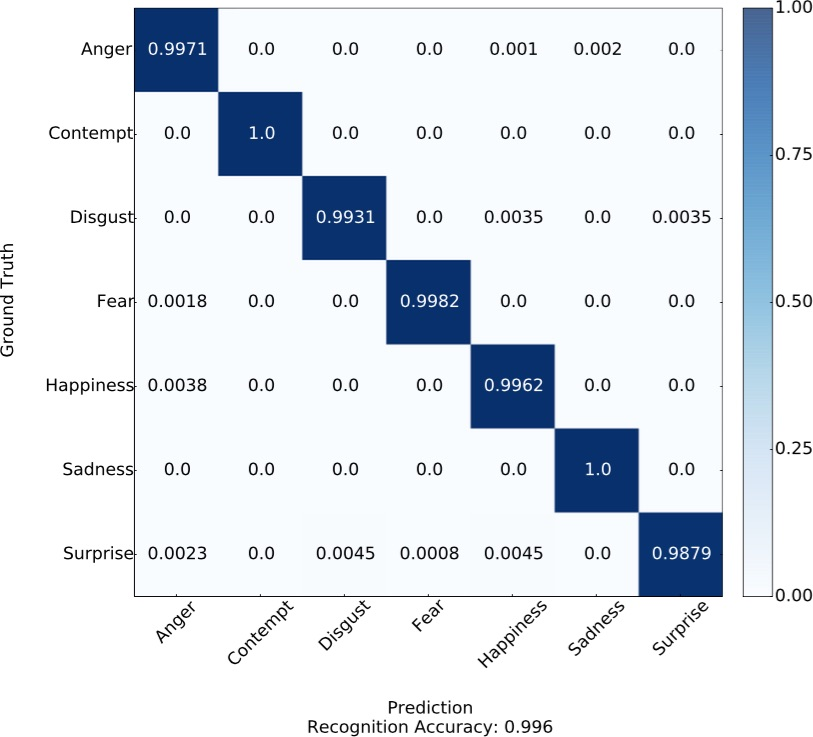
\includegraphics[width=0.9\columnwidth]{Fig6}
\caption{The confusion matrix of the averaged 10-fold cross-validation on the CKP Dataset. The lowest accuracy is achieved by the emotion \textit{Surprise} with $98.79\%$ while \textit{Contempt}/\textit{Sadness} are both recognized with $100\%$.}
\label{fig:ckp_conf}
\end{subfigure}
\hspace{0.05\textwidth}
\begin{subfigure}[b]{0.46\textwidth}
\centering
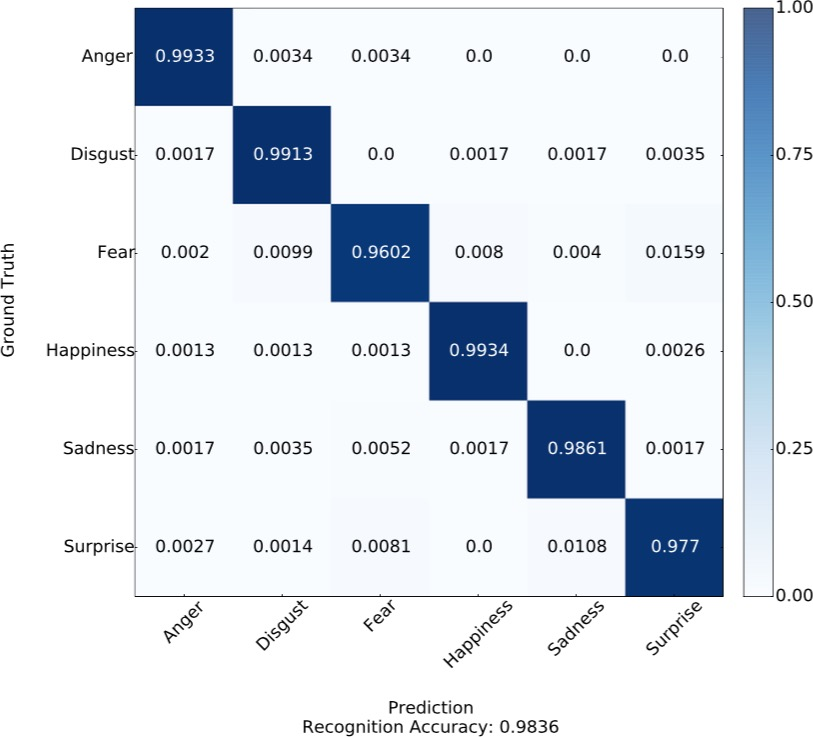
\includegraphics[width=0.9\columnwidth]{Fig7}
\caption{The confusion matrix of the averaged 10-fold cross-validation on the MMI Dataset. The lowest accuracy is achieved by the emotion \textit{Fear} with $93.75\%$. \textit{Happiness} is recognized with $98.21\%$.\\~}
\label{fig:mmi_conf}
\end{subfigure}
\end{figure*}


\paraV
\paragraph{\textbf{MMI}}
The MMI Database contains videos of people showing emotions. From each video the 20 frames, which represent the content of the video the most, have been extracted fully automatically. The first two of these frames have been discarded since they provide neutral expressions. \\
To determine the frames, the difference between grayscale consecutive frames was calculated. To compensate noise the images have been smoothed using a Gaussian filter before calculation. To find the 20 most representative images, changes which occur in a small timeframe, should only be represented by a single image. This was achieved by iterating over the differences using a maximum filter with decreasing filter size until 20 frames have been found. In total 3740 images have been extracted.\\
The original images were then used for training and testing. A 10-fold cross-validation has been applied. The average accuracy is 98.63\%. This is better than the accuracies achieved by Wang and Yin~\cite{Wang:2007:STM:1287852.1288093} (Table~\ref{tab:mmi_results}). To our knowledge they have been the only ones to evaluate the MMI database on Emotions instead of Action Units. The results of the proposed approach are depicted in the Confusion Matrix in Fig.~\ref{fig:mmi_conf}. In the figure it is shown that the accuracy for \textit{Fear} is the lowest with 93.75\% while \textit{Happiness} is almost perfectly recognized with 98.21\%. \textit{Fear} and \textit{Surprise} are the emotions confused the most. 

\begin{table}[!ht]
\caption{This Table summarizes the current state of the art in emotion recognition on the MMI database (Section~\ref{sec:mmi}).}
\label{tab:mmi_results}
\centering
\begin{tabular}{l|c|c}
\hline
Author & Method & Accuracy \\
\hline
Wang and Yin~\cite{Wang:2007:STM:1287852.1288093} & LDA & 93.33\%\\
Wang and Yin~\cite{Wang:2007:STM:1287852.1288093} & QDC & 92.78\%\\
Wang and Yin~\cite{Wang:2007:STM:1287852.1288093} & NBC & 85.56\%\\
\hline
DeXpression (Proposed) & &98.63\% \\
\hline
\end{tabular}

\end{table}
